\usetikzlibrary{calc}
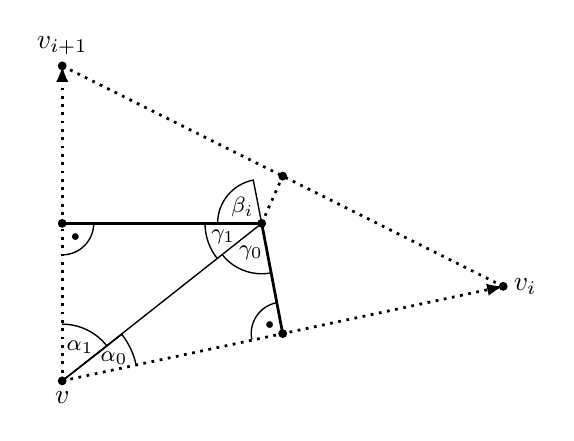
\begin{tikzpicture}[>=latex, line width=1pt, scale=0.8]
%coords
%center
\coordinate (C) at (3.1666,2.5);
%vertices
\coordinate (V) at (0,0);
\coordinate (Vi) at (7,1.5);
\coordinate (Vi1) at (0,5);
%edge centers
\coordinate (CCi) at (3.5,0.75);
\coordinate (CCi1) at (0,2.5);
\coordinate (CCii1) at (3.5,3.25);

%nodes
\fill (V) node[below] {\(v\)} circle(2pt);
\fill (Vi) node[right] {\(v_i\)} circle(2pt);
\fill (Vi1) node[above] {\(v_{i+1}\)} circle(2pt);
\fill (C) circle(2pt);
\fill (CCi) circle(2pt);
\fill (CCi1) circle(2pt);
\fill (CCii1) circle(2pt);

%lines
%edges
\draw[style=dotted, ->] (V) -- (Vi);
\draw[style=dotted] (Vi) -- (Vi1);
\draw[style=dotted, ->] (V) -- (Vi1);
%voronoi edges
\draw (CCi) -- (C);
\draw (C) -- (CCi1);
\draw[style=dotted] (C) -- (CCii1);
%nonelementary dual edge 
\draw[line width=0.5pt] (C) -- (V);

%angles
%rightangles
\draw[line width=0.5pt] (CCi) -- +(101:0.5) arc (101:191:0.5);
\node at ($(CCi)+(146:0.25)$) {\tiny\(\bullet\)};
\draw[line width=0.5pt] (CCi1) -- +(0:0.5) arc (0:-90:0.5);
\node at ($(CCi1)+(315:0.3)$) {\tiny\(\bullet\)};
%beta
\draw[line width=0.5pt] (C) -- +(101:0.7) arc (101:180:0.7);
\node at ($(C)+(140:0.4)$) {\footnotesize\(\beta_i\)};
%gammas
\draw[line width=0.5pt] (C) -- +(180:0.9) arc (180:219:0.9);
\node at ($(C)+(199.5:0.65)$) {\footnotesize\(\gamma_1\)};
\draw[line width=0.5pt] (C) -- +(281:0.8) arc (281:219:0.8);
\node at ($(C)+(250:0.5)$) {\footnotesize\(\gamma_0\)};
%alphas
\draw[line width=0.5pt] (V) -- +(38:0.9) arc (38:90:0.9);
\node at ($(V)+(62:0.6)$) {\footnotesize\(\alpha_1\)};
\draw[line width=0.5pt] (V) -- +(38:1.2) arc (38:12:1.2);
\node at ($(V)+(24:0.9)$) {\footnotesize\(\alpha_0\)};

\end{tikzpicture}